\documentclass[11pt]{article}

\usepackage[margin=1.1in]{geometry}
\usepackage{amsmath,amssymb}
\usepackage{booktabs}
\usepackage{tikz}
\usepackage[colorlinks=true,linkcolor=blue!60!black,citecolor=green!40!black,urlcolor=blue!60!black]{hyperref}

\newcommand{\mat}[1]{\mathbf{#1}}
\newcommand{\vect}[1]{\mathbf{#1}}
\newcommand{\R}{\mat{R}}
\newcommand{\K}{\mat{K}}
\newcommand{\F}{\mat{F}}
\newcommand{\E}{\mat{E}}
\newcommand{\PP}{\mat{P}}
\newcommand{\X}{\vect{X}}
\newcommand{\x}{\vect{x}}
\newcommand{\tv}{\vect{t}}
\newcommand{\Cv}{\vect{C}}
\newcommand{\code}[1]{\texttt{#1}}

\title{\textsc{multiview}: A Portable C99 System for Two-Camera\\
Scene Analysis and 3D Model Extraction}
\author{Project documentation --- v0.1.0}
\date{August 2, 2026}

\begin{document}
\maketitle

\begin{abstract}
\textsc{multiview} is a small, dependency-free C99 library for metric scene
analysis and 3D model extraction from the synchronized video streams of
\emph{two stationary, calibrated cameras} observing an overlapping volume,
optionally augmented by an unordered collection of still photographs and, in a
later stage, range-finder measurements. This document is self-contained: it
states what the system can do today (\autoref{sec:capabilities}), develops the
underlying multiview-geometry theory from the camera model up
(\autoref{sec:camera}--\autoref{sec:stereo}), describes the numerical choices
made in the implementation (\autoref{sec:numerics}), and reports first
quantitative results on a controlled synthetic scene
(\autoref{sec:results}). It is written to support later self-study and
incremental development of the code base in a controlled environment: every
claim in \autoref{sec:results} is reproducible from the deterministic test
programs in the repository.
\end{abstract}

\tableofcontents

%----------------------------------------------------------------------
\section{Introduction and capabilities}
\label{sec:capabilities}

The target deployment is deliberately narrow and fully under our control: two
cameras are rigidly mounted, their intrinsic and extrinsic calibration is
known (or measured once, offline), and both observe the same working volume.
Video from this rig is processed frame by frame; because the cameras do not
move, all geometric quantities that depend only on the rig --- projection
matrices, the fundamental matrix, the rectifying homographies --- are computed
\emph{once} and reused for every frame, which is the central efficiency win of
the stationary-rig assumption.

The implemented core (v0.1.0) provides:
\begin{enumerate}
  \item a calibrated pinhole camera model with Brown radial--tangential lens
        distortion, forward projection and ray back-projection
        (\autoref{sec:camera});
  \item exact two-view epipolar geometry from the calibration, and the
        normalized 8-point algorithm to estimate or verify it from image
        correspondences (\autoref{sec:epipolar});
  \item $N$-view linear triangulation of corresponding image points into
        metric 3D, with reprojection-error reporting
        (\autoref{sec:triangulation});
  \item planar stereo rectification of the pair, and dense correspondence by
        block matching with sub-pixel refinement, giving per-pixel depth
        (\autoref{sec:stereo});
  \item point-cloud assembly and PLY export for inspection in standard mesh
        tools, plus minimal PGM image I/O (\autoref{sec:models}).
\end{enumerate}

Planned extensions --- structure-from-motion over an auxiliary photo
collection and fusion of range-finder data --- are designed but not yet
implemented; their theory and integration points are described in
\autoref{sec:extensions} so that the code can grow into them without
rearchitecting.

\paragraph{Design constraints.} The library is strict C99 with no
dependencies beyond \code{libm}, row-major \code{double} arrays throughout,
and fully deterministic (no clocks, no ambient randomness; the demo uses a
fixed-seed generator). This keeps it portable from desktop to embedded
targets, and keeps every experiment repeatable --- a prerequisite for the
controlled-environment, learning-oriented use the project is intended for.

%----------------------------------------------------------------------
\section{System overview}
\label{sec:overview}

\begin{table}[h]
\centering
\begin{tabular}{lll}
\toprule
Module & Header & Responsibility \\
\midrule
\code{mat}         & \code{mv/mat.h}         & small dense linear algebra, Jacobi SVD, null vectors \\
\code{cam}         & \code{mv/cam.h}         & camera model, projection, rays, distortion \\
\code{epipolar}    & \code{mv/epipolar.h}    & $\F$ from calibration; normalized 8-point; $\E$ \\
\code{triangulate} & \code{mv/triangulate.h} & $N$-view DLT triangulation, reprojection RMS \\
\code{rectify}     & \code{mv/rectify.h}     & Fusiello rectification, disparity$\to$depth \\
\code{stereo}      & \code{mv/stereo.h}      & dense block matching (SAD, sub-pixel) \\
\code{img}         & \code{mv/img.h}         & PGM (P5) image I/O \\
\code{cloud}       & \code{mv/cloud.h}       & point cloud container, PLY export \\
\bottomrule
\end{tabular}
\caption{Module layout. \code{mv/mv.h} is the umbrella header.}
\label{tab:modules}
\end{table}

The per-frame processing pipeline is:
\[
\underbrace{\text{2 video frames}}_{\text{capture}}
\;\rightarrow\;
\underbrace{\text{undistort}}_{\code{cam}}
\;\rightarrow\;
\underbrace{\text{rectify}}_{\code{rectify}}
\;\rightarrow\;
\underbrace{\text{dense match}}_{\code{stereo}}
\;\rightarrow\;
\underbrace{\text{depth / triangulate}}_{\code{triangulate}}
\;\rightarrow\;
\underbrace{\text{cloud accumulation}}_{\code{cloud}}
\]
Sparse operation (feature correspondences instead of dense matching) uses the
same chain with \code{epipolar} providing the correspondence-validation
gate. Because the rig is static, temporal accumulation over video frames is a
simple union of per-frame clouds in the fixed world frame; moving objects
appear as temporally inconsistent points and can be segmented by comparing
frames, which is the entry point for scene \emph{analysis} beyond
reconstruction.

%----------------------------------------------------------------------
\section{Camera model and calibration}
\label{sec:camera}

A camera is modeled as a pinhole with intrinsic matrix
\begin{equation}
\K = \begin{pmatrix} f_x & s & c_x \\ 0 & f_y & c_y \\ 0 & 0 & 1 \end{pmatrix},
\label{eq:K}
\end{equation}
rotation $\R$ and translation $\tv$ mapping world points into the camera
frame, $\X_c = \R\X + \tv$; the camera center is $\Cv = -\R^{\!\top}\tv$. A
world point projects to the homogeneous pixel
\begin{equation}
\x \;\simeq\; \PP \begin{pmatrix}\X\\1\end{pmatrix},
\qquad
\PP = \K\,[\,\R \mid \tv\,],
\label{eq:pinhole}
\end{equation}
where $\simeq$ denotes equality up to scale \cite{HartleyZisserman2004}.
Real lenses deviate from \eqref{eq:pinhole}; we use the Brown model on
normalized coordinates $(x,y)$, $r^2 = x^2{+}y^2$:
\begin{equation}
\begin{aligned}
x_d &= x\,(1 + k_1 r^2 + k_2 r^4 + k_3 r^6) + 2p_1 xy + p_2(r^2 + 2x^2),\\
y_d &= y\,(1 + k_1 r^2 + k_2 r^4 + k_3 r^6) + p_1(r^2 + 2y^2) + 2p_2 xy.
\end{aligned}
\label{eq:distortion}
\end{equation}
Back-projection inverts \eqref{eq:distortion} by fixed-point iteration
(20 iterations suffice for the moderate distortions of machine-vision
lenses) and returns the ray $\Cv + s\,\vect{d}$, $s>0$.

Calibration itself is treated as an \emph{input}: the rig is calibrated once
offline with standard planar-target methods \cite{Zhang2000,Tsai1987}, and
the resulting $(\K,\R,\tv,k_{1..5})$ per camera is what
\autoref{sec:epipolar}--\autoref{sec:stereo} consume. The stationary rig
makes this a one-time cost and removes online self-calibration from the
critical path.

%----------------------------------------------------------------------
\section{Two-view epipolar geometry}
\label{sec:epipolar}

\begin{figure}[h]
\centering
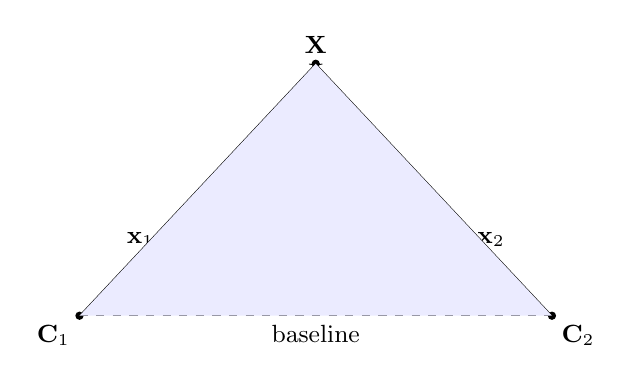
\begin{tikzpicture}[scale=1.0]
  % camera centers
  \coordinate (C1) at (0,0);
  \coordinate (C2) at (6,0);
  \coordinate (X)  at (3,3.2);
  % image planes
  \draw[thick] (0.6,0.2) -- (1.6,1.4) node[midway,below right,font=\small] {$\pi_1$};
  \draw[thick] (5.4,0.2) -- (4.4,1.4) node[midway,below left,font=\small] {$\pi_2$};
  % rays
  \draw[->] (C1) -- (X) node[above,font=\small] {$\X$};
  \draw[->] (C2) -- (X);
  % baseline
  \draw[dashed] (C1) -- (C2) node[midway,below,font=\small] {baseline};
  % epipolar points
  \fill (C1) circle (1.5pt) node[below left,font=\small] {$\Cv_1$};
  \fill (C2) circle (1.5pt) node[below right,font=\small] {$\Cv_2$};
  \fill (X) circle (1.5pt);
  \fill (1.07,0.76) circle (1.2pt) node[above left,font=\small] {$\x_1$};
  \fill (4.93,0.76) circle (1.2pt) node[above right,font=\small] {$\x_2$};
  % epipolar plane shading
  \fill[blue!8] (C1) -- (X) -- (C2) -- cycle;
\end{tikzpicture}
\caption{Epipolar geometry: the camera centers $\Cv_1,\Cv_2$ and the scene
point $\X$ span the epipolar plane (shaded); its intersections with the image
planes $\pi_1,\pi_2$ are the corresponding epipolar lines on which $\x_1$ and
$\x_2$ must lie.}
\label{fig:epipolar}
\end{figure}

Corresponding pixels of the two views are linked by the fundamental matrix
$\F$ through the epipolar constraint
\begin{equation}
\x_2^{\!\top}\,\F\,\x_1 = 0,
\label{eq:epiconstraint}
\end{equation}
with $\F$ of rank 2; the line $\boldsymbol{\ell}_2 = \F\x_1$ is the locus in
image 2 of possible matches of $\x_1$ (\autoref{fig:epipolar}). For
\emph{calibrated} views the essential matrix
$\E = \K_2^{\!\top}\F\,\K_1 = [\tv]_\times\R$ carries the same constraint in
normalized coordinates \cite{LonguetHiggins1981}.

Because our rig is calibrated, $\F$ is available in closed form,
\begin{equation}
\F = [\,e_2\,]_\times\, \PP_2\, \PP_1^{+},
\qquad e_2 = \PP_2\begin{pmatrix}\Cv_1\\1\end{pmatrix},
\label{eq:fundamental}
\end{equation}
where $\PP_1^{+}$ is the pseudo-inverse of $\PP_1$
\cite{HartleyZisserman2004}. The system computes \eqref{eq:fundamental} once
at start-up and uses it for \emph{correspondence gating}: any candidate match
whose symmetric epipolar distance exceeds a threshold is rejected before
triangulation.

Independently, $\F$ can be \emph{estimated} from $n\ge 8$ point
correspondences by the normalized 8-point algorithm \cite{Hartley1997}: each
pair contributes one linear equation in the entries of $\F$, the points being
first translated and scaled to centroid $0$ and RMS radius $\sqrt2$
(normalization is essential for conditioning, see \autoref{sec:numerics});
the solution is the smallest right singular vector of the design matrix,
followed by rank-2 enforcement via SVD. In this system the estimator serves
two purposes: (i) \emph{health monitoring} --- if the estimate from live
correspondences drifts from the calibrated \eqref{eq:fundamental}, the rig
has been bumped or the calibration is stale; (ii) bootstrapping geometry for
\emph{uncalibrated} auxiliary photos (\autoref{sec:extensions}). On
contaminated correspondence sets the estimator is wrapped in a RANSAC loop
\cite{FischlerBolles1981} (planned with the feature layer).

%----------------------------------------------------------------------
\section{Triangulation}
\label{sec:triangulation}

Given observations $\x^{(v)} = (u_v, w_v)$ of the same point in $N\ge2$ views
with projection matrices $\PP^{(v)}$, each view contributes two linear
equations obtained by eliminating the projective scale from
\eqref{eq:pinhole}:
\begin{equation}
\begin{pmatrix}
u_v\,\PP^{(v)}_{3,:} - \PP^{(v)}_{1,:}\\[2pt]
w_v\,\PP^{(v)}_{3,:} - \PP^{(v)}_{2,:}
\end{pmatrix}
\begin{pmatrix}\X\\1\end{pmatrix} = \vect{0},
\label{eq:dlt}
\end{equation}
and stacking all views gives a $2N\times4$ homogeneous system whose
least-squares solution (smallest right singular vector, then
dehomogenization) is the DLT triangulation \cite{HartleyZisserman2004}. The
implementation accepts any $N\ge2$, so still photographs registered into the
rig frame (\autoref{sec:extensions}) simply extend the same call. DLT
minimizes an algebraic residual; the gold-standard reprojection-optimal
two-view method of Hartley--Sturm \cite{HartleySturm1997} is a planned
refinement, worthwhile mainly for wide-baseline auxiliary views. The library
reports the RMS reprojection error of every triangulated point, which is the
quantity an eventual bundle adjustment would minimize \cite{Triggs2000}.

%----------------------------------------------------------------------
\section{Rectification and dense stereo}
\label{sec:stereo}

For dense per-pixel depth the pair is first \emph{rectified}: both cameras
are rotated (synthetically, about their centers) onto a common orientation
whose $x$ axis is the baseline, so epipolar lines become identical image rows
and correspondence search collapses to 1D. We use the compact algorithm of
Fusiello, Trucco and Verri \cite{Fusiello2000}: the new rotation has rows
$(\vect{x},\vect{y},\vect{z})$ with $\vect{x}$ the unit baseline,
$\vect{y}=\vect{k}\times\vect{x}$ ($\vect{k}$ the old optical axis of camera
1) and $\vect{z}=\vect{x}\times\vect{y}$; both views share the averaged
intrinsics with zero skew, and the pixel maps are the homographies
$\mat{H}_i = \K_{\mathrm{new}}\R_{\mathrm{new}}\R_i^{\!\top}\K_i^{-1}$.
Since the rig is stationary, $\mat{H}_1,\mat{H}_2$ are computed once and each
video frame is warped by table lookup.

On the rectified pair, dense correspondence is found by block matching:
for each left pixel the sum of absolute differences (SAD) over a
$(2w{+}1)^2$ window is minimized along the corresponding right row over a
disparity range, followed by sub-pixel refinement by parabolic interpolation
of the cost around the minimum. This is the classic local baseline method in
the taxonomy of Scharstein and Szeliski \cite{ScharsteinSzeliski2002} ---
chosen deliberately: it is simple, portable, trivially parallel, and its
failure modes (textureless regions, occlusions, repetitive patterns) are
well understood, giving a controlled baseline against which future matchers
(rank/census transforms, semi-global aggregation) can be measured within the
same harness.

Matched disparity $d$ converts to metric depth by
\begin{equation}
Z = \frac{f\,B}{d},
\label{eq:depth}
\end{equation}
with $f$ the shared rectified focal length (pixels) and $B$ the baseline.
Differentiating \eqref{eq:depth} gives the expected depth uncertainty
\begin{equation}
\sigma_Z \;=\; \frac{Z^2}{f\,B}\,\sigma_d,
\label{eq:deptherr}
\end{equation}
for disparity noise $\sigma_d$ --- the quadratic growth with $Z$ is the
fundamental accuracy law of the rig and is verified experimentally in
\autoref{sec:results}.

%----------------------------------------------------------------------
\section{From depth to models}
\label{sec:models}

Every depth estimate back-projects to a 3D point in the fixed world frame;
points are accumulated in a growable cloud with optional per-point color and
exported as ASCII PLY, directly loadable in MeshLab, CloudCompare or Blender
for inspection. Over a video sequence the static-rig assumption makes
accumulation a union in a common frame; per-point temporal statistics
(persistence, variance) separate static structure from moving objects. The
planned meshing path is classical: volumetric range-image fusion
\cite{CurlessLevoy1996} or Poisson surface reconstruction
\cite{Kazhdan2006} over the accumulated cloud; both consume exactly the
oriented-point data the pipeline produces, so they attach cleanly as later
modules.

%----------------------------------------------------------------------
\section{Planned extensions}
\label{sec:extensions}

\subsection{Auxiliary photo collections}
\label{sec:photos}

Still photographs of the same volume --- arbitrary viewpoints, possibly a
different camera --- densify coverage and fill occlusions. The integration
path follows the structure-from-motion recipe of Photo Tourism
\cite{Snavely2006}: detect scale-invariant features \cite{Lowe2004} in the
photos \emph{and} in the two calibrated video frames; match with a RANSAC
gate \cite{FischlerBolles1981}; register each photo to the rig's world frame
by resection from matches against already-triangulated points; then
re-triangulate all tracks with the registered views via the existing
$N$-view DLT (\autoref{sec:triangulation}); finally refine everything with
bundle adjustment \cite{Triggs2000}. The two calibrated cameras anchor the
metric scale --- the classic scale ambiguity of pure SfM does not arise.
Dense multiview stereo over the registered set (e.g.\ patch-based methods
\cite{FurukawaPonce2010}) is a further optional stage.

\subsection{Range-finder fusion}
\label{sec:range}

A range finder (laser/ToF) contributes sparse but metrically strong depth.
Two integration modes are planned: (i) if the range finder is rigidly mounted
and extrinsically calibrated to the rig, each range sample is simply another
world-frame point with small $\sigma_Z$, fused into the cloud with
inverse-variance weights; (ii) if it produces an independent scan, the scan
is registered to the vision cloud by closed-form absolute orientation
\cite{Horn1987} initialized correspondence-free and refined with ICP
\cite{BeslMcKay1992}. In both modes the range data additionally serves as a
ground-truth audit of the stereo depth law \eqref{eq:deptherr}.

%----------------------------------------------------------------------
\section{Numerical implementation notes}
\label{sec:numerics}

All decompositions reduce to one kernel: a one-sided (Hestenes) Jacobi SVD
\cite{GolubVanLoan2013} for $m\ge n$ matrices, $n\le9$ in every present use
(design matrices of \eqref{eq:dlt} and the 8-point system). Jacobi SVD was
chosen over Golub--Kahan bidiagonalization for its simplicity ($\sim$100
lines, no workspace queries), unconditional convergence, and excellent
relative accuracy on small matrices; its $O(mn^2)$-per-sweep cost is
irrelevant at these sizes. Homogeneous solutions ($\F$, DLT points) are the
right singular vector of the smallest singular value; rank-2 enforcement for
$\F$ zeroes the smallest singular value and recomposes.

Conditioning is handled where it matters: the 8-point design matrix mixes
terms of order $1$, $u$, and $u^2$ ($u\sim10^2$ pixels), giving condition
numbers around $10^8$ unnormalized; Hartley normalization
\cite{Hartley1997} (centroid $0$, RMS radius $\sqrt2$) reduces this to
$O(10)$ and is applied always, with the result denormalized as
$\F = \mat{T}_2^{\!\top}\hat\F\,\mat{T}_1$. All fundamental matrices are
canonicalized (unit Frobenius norm, largest-magnitude entry positive) so
that analytic and estimated matrices are directly comparable --- this is what
makes the drift monitor of \autoref{sec:epipolar} a plain matrix norm.

The code is strict C99 (\code{-std=c99 -pedantic -Wall -Wextra} clean),
depends only on \code{libm}, allocates only in unavoidable places (design
matrices, images, clouds), and contains no hidden state except the demo's
seeded generator. Determinism is treated as a feature: identical inputs give
bit-identical outputs across runs, so every regression is reproducible.

%----------------------------------------------------------------------
\section{Basic results}
\label{sec:results}

Two validation programs accompany the library. \code{tests/test\_mv.c}
checks exact properties on noiseless data (19 assertions: SVD reconstruction
and orthonormality, inverse correctness, center recovery, ray/projection
consistency, \eqref{eq:epiconstraint} to $10^{-8}$, exact triangulation
recovery, row alignment after rectification); all pass.
\code{demo/synthetic.c} is the first controlled experiment: two cameras with
$f=800$\,px, $640\times480$ images, baseline $B=0.5$\,m, the second camera
yawed $6^\circ$ inward, observing 250 points drawn uniformly in a
$2\times1.5$\,m window at depths $3.5$--$6$\,m; projections are corrupted
with Gaussian noise $\sigma=0.3$\,px per coordinate (seed fixed).
\autoref{tab:results} summarizes the outcome.

\begin{table}[h]
\centering
\begin{tabular}{lr}
\toprule
Quantity & Value \\
\midrule
points visible in both views                       & $250/250$ \\
$\|\F_{\text{analytic}}-\F_{\text{8-point}}\|_F$ (unit-norm)  & $4.5\times10^{-3}$ \\
mean symmetric epipolar distance (analytic $\F$)   & $0.345$ px \\
mean symmetric epipolar distance (8-point $\F$)    & $0.341$ px \\
triangulation RMS 3D error                         & $0.0265$ m \\
triangulation max 3D error                         & $0.0876$ m \\
RMS reprojection error                             & $0.218$ px \\
mean row misalignment $|v_1-v_2|$ before rectification & $0.764$ px \\
mean row misalignment after rectification          & $0.0$ px \\
\bottomrule
\end{tabular}
\caption{Synthetic experiment, seed 42 (reproduce with \code{make demo}).}
\label{tab:results}
\end{table}

The numbers are consistent with theory. The epipolar residual
$\approx0.34$\,px matches the injected noise level. The depth-error law
\eqref{eq:deptherr} with $\bar Z\approx4.7$\,m, $fB=400$\,px$\cdot$m and
disparity noise $\sigma_d=\sqrt2\,\sigma\approx0.42$\,px predicts
$\sigma_Z\approx2.3$\,cm; the measured RMS 3D error of $2.65$\,cm (which
also contains the smaller lateral components) agrees, confirming that the
implementation performs at the noise floor of the geometry rather than being
implementation-limited. The 8-point estimate reproduces the calibrated
$\F$ to $4.5\times10^{-3}$ in Frobenius norm from noisy data --- tight
enough to serve as the calibration-drift monitor of \autoref{sec:epipolar}.
The reconstructed cloud is written to \code{out\_cloud.ply} for visual
inspection.

%----------------------------------------------------------------------
\section{Roadmap}
\label{sec:roadmap}

In dependency order: (1) feature detection/description and robust matching
(enables live correspondences, RANSAC-gated by \autoref{sec:epipolar});
(2) image warping by the rectifying homographies with bilinear resampling,
closing the dense video path end-to-end; (3) temporal cloud statistics for
static/moving segmentation (\autoref{sec:models}); (4) photo-collection
registration (\autoref{sec:photos}); (5) Hartley--Sturm optimal
triangulation and bundle adjustment; (6) range-finder fusion
(\autoref{sec:range}); (7) meshing. Each step lands as a new module behind
the same conventions (\autoref{tab:modules}) with its own noiseless-exact
tests and a synthetic experiment extending \autoref{tab:results}.

\bibliographystyle{alpha}
\bibliography{refs}

\end{document}
